%%%%%%%%%%%%%%%%%%%%%%%%%%%%%%%%%%%%%%%%%
% Beamer Presentation
% LaTeX Template
% Version 1.0 (10/11/12)
%
% This template has been downloaded from:
% http://www.LaTeXTemplates.com
%
% License:
% CC BY-NC-SA 3.0 (http://creativecommons.org/licenses/by-nc-sa/3.0/)
%
%%%%%%%%%%%%%%%%%%%%%%%%%%%%%%%%%%%%%%%%%

%----------------------------------------------------------------------------------------
%	PACKAGES AND THEMES
%----------------------------------------------------------------------------------------

\documentclass[9pt]{beamer}
\usepackage{CJK}
\usepackage{ctex}
\usepackage{graphicx}
\usepackage{subfigure}
\usepackage{longtable}
\usepackage{rotating}
\usepackage{multirow}
\usepackage{algorithm}
\usepackage{algorithmic}
\usepackage{mathtools}
\usepackage{animate}
%\usepackage{media9}
%% A LATEX package for embedding interactive Adobe Flash (SWF) and 3D files (Adobe U3D & PRC) as well as video and sound files or streams (FLV, MP4/H.246, MP3) into PDF documents with Adobe Reader-9/X
%compatibility.
\renewcommand{\algorithmicrequire}{\textbf{Input:}}   %Use Input in the format of Algorithm
\renewcommand{\algorithmicensure}{\textbf{Output:}}  %UseOutput in the format of Algorithm
\newcommand{\e}[1]{\ensuremath{\times 10^{#1}}}
%\mode<presentation>{\usetheme{Madrid}}

\mode<presentation> {

% The Beamer class comes with a number of default slide themes
% which change the colors and layouts of slides. Below this is a list
% of all the themes, uncomment each in turn to see what they look like.

%\usetheme{default}
%\usetheme{AnnArbor}
%\usetheme{Antibes}
%\usetheme{Bergen}
%\usetheme{Berkeley}
%\usetheme{Berlin}
%\usetheme{Boadilla}
%\usetheme{CambridgeUS}
%\usetheme{Copenhagen}
%\usetheme{Darmstadt}
%\usetheme{Dresden}
%\usetheme{Frankfurt}
%\usetheme{Goettingen}
%\usetheme{Hannover}
%\usetheme{Ilmenau}
%\usetheme{JuanLesPins}
%\usetheme{Luebeck}
\usetheme{Madrid}
%\usetheme{Malmoe}
%\usetheme{Marburg}
%\usetheme{Montpellier}
%\usetheme{PaloAlto}
%\usetheme{Pittsburgh}
%\usetheme{Rochester}
%\usetheme{Singapore}
%\usetheme{Szeged}
%\usetheme{Warsaw}

% As well as themes, the Beamer class has a number of color themes
% for any slide theme. Uncomment each of these in turn to see how it
% changes the colors of your current slide theme.

%\usecolortheme{albatross}
\usecolortheme{beaver}
%\usecolortheme{beetle}
%\usecolortheme{crane}
%\usecolortheme{dolphin}
%\usecolortheme{dove}
%\usecolortheme{fly}
%\usecolortheme{lily}
%\usecolortheme{orchid}
%\usecolortheme{rose}
%\usecolortheme{seagull}
%\usecolortheme{seahorse}
%\usecolortheme{whale}
%\usecolortheme{wolverine}

%\setbeamertemplate{footline} % To remove the footer line in all slides uncomment this line
%\setbeamertemplate{footline}[page number] % To replace the footer line in all slides with a simple slide count uncomment this line

%\setbeamertemplate{navigation symbols}{} % To remove the navigation symbols from the bottom of all slides uncomment this line
}

\usepackage{graphicx} % Allows including images
\usepackage{booktabs} % Allows the use of \toprule, \midrule and \bottomrule in tables
\begin{document}
\begin{CJK*}{GBK}{kai}
%----------------------------------------------------------------------------------------
%	TITLE PAGE
%----------------------------------------------------------------------------------------

\title[Machine Learning]{Estimating Probabilities from data} % The short title appears at the bottom of every slide, the full title is only on the title page

%\author{Fuhao Zou(�޸���)}
\author{Fuhao Zou(�޸���)} % Your name
%\logo{%
%   
\includegraphics[scale=.2]{logo.pdf}\hspace*{4.75cm}~%
%   
\includegraphics[scale=.2]{logo.jpg}\hspace*{0.75cm}%
%   }
%\pgfdeclareimage[width=1cm]{hust}{logo.pdf}
%\logo{\pgfuseimage{hust}{\vspace{-10pt}}}
\titlegraphic{
\includegraphics[width=1.3cm]{logo.pdf}}
\institute[IEC, HUST] % Your institution as it will appear on the bottom of every slide, may be shorthand to save space
{
Intelligent and Embedded Computing Lab��\\
                   Huazhong University of Science \& Technology \\ % Your institution for the title page
\medskip
\textit{fuhao\_zou@hust.edu.cn} % Your email address
}

\date{2019��04��13��} % Date, can be changed to a custom date
%====================================================
\frame{\titlepage}

\frame{\frametitle{Table of contents}\tableofcontents}

\AtBeginSection[]
{
\begin{frame}{Table of Contents}
\tableofcontents[currentsection]
\end{frame}
}

%------------------------------------------------
%------------------------------------------------
\section{Introduction}
%------------------------------------------------
\subsection{Bayes Optimal classifier:}
\begin{frame}
\frametitle{Bayes Optimal classifier:}
\begin{block}{Idea:}
	If we are provided with \mathrm{P}(X,Y) we can predict the most likely label for x, formally $argmax_y$P(y$|$x). It is therefore worth considering if we can estimate P(X,Y) directly from the training data. If this is possible (to a good approximation) we could then use the Bayes Optimal classifier in practice on our estimate of P(X,Y).
\end{block}
	In fact, many supervised learning can be viewed as estimating P(X,Y). Generally, they fall into two categories:	
\begin{itemize}
	\item When we estimate P(X,Y)=P(X$|$Y)P(Y), then we call it generative learning
	\item When we only estimate P(Y$|$X) directly, then we call it discriminative learning.	
\end{itemize}
	So how can we estimated probability distributions from samples?
\end{frame}
%------------------------------------------------
% \begin{frame}
% \frametitle{Formal definition of k-NN:}
% \begin{block}{Formal definition}
% \begin{itemize}
% \item Test point: $\mathbf{x}$
% \item Denote the set of the $k$ nearest neighbors of $\mathbf{x}$ as $S_\mathbf{x}$. Formally $S_\mathbf{x}$ is defined as $S_\mathbf{x}\subseteq {D}$ s.t. $|S_\mathbf{x}|=k$ and $\forall(\mathbf{x}',y')\in D\backslash S_\mathbf{x}$,
% \[\text{dist}(\mathbf{x},\mathbf{x}')\ge\max_{(\mathbf{x}'',y'')\in S_\mathbf{x}} \text{dist}(\mathbf{x},\mathbf{x}''),\]
% (i.e. every point in $D$ but \textit{not} in $S_\mathbf{x}$ is at least as far away from $\mathbf{x}$ as the furthest point in $S_\mathbf{x}$).
% We can then define the classifier $h()$ as a function returning the most common label in $S_\mathbf{x}$:
% \[h(\mathbf{x})=\text{mode}(\{y'':(\mathbf{x}'',y'')\in S_\mathbf{x}\}),\]
% where $\text{mode}(\cdot)$ means to select the label of the highest occurrence.
% \end{itemize}
% \end{block}
% \end{frame}

%------------------------------------------------
% \subsection{Example}
% \begin{frame}
% \frametitle{A binary classification example}
% \begin{figure}[h]
% 	\centering
% 	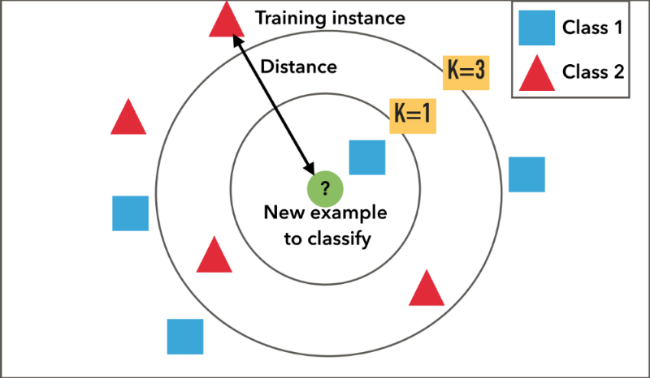
\includegraphics[scale=0.4]{note0}
% 	\caption{Example of k-NN classification. The test sample (inside circle) should be classified either to the first class of blue squares or to the second class of red triangles. If k = 3 (outside circle) it is assigned to the second class because there are 2 triangles and only 1 square inside the inner circle. If, for example k = 5 it is assigned to the first class (3 squares vs. 2 triangles outside the outer circle).}
% \end{figure}
% \end{frame}
%------------------------------------------------
\section{Maximum Likelihood Estimation (MLE)}
%------------------------------------------------
\subsection{Simple scenario: coin toss}
\begin{frame}
\frametitle{Simple scenario: coin toss}
\begin{block}{Question}
	Suppose you find a coin and it's ancient and very valuable. Naturally, you ask yourself, "What is the probability that this coin comes up heads when I toss it?" You toss it n=10 times and obtain the following sequence of outcomes: D={H,T,T,H,H,H,T,T,T,T}. Based on these samples, how would you estimate P(H)? 
\end{block}

We observed $n_H$=4 heads and $n_T$=6 tails. So, intuitively,

$$P(H)\approx \dfrac{n_H}{n_H+n_T}=\dfrac{4}{10}=0.4$$

Can we derive this more formally?

\end{frame}
%------------------------------------------------
\subsection{Maximum Likelihood Estimation (MLE)}
\begin{frame}
\frametitle{Maximum Likelihood Estimation (MLE)}
\begin{block}{MLE}
	The estimator we just mentioned is the Maximum Likelihood Estimate (MLE). For MLE you typically proceed in two steps: 

	First, you make an explicit modeling assumption about what type of distribution your data was sampled from. 

	Second, you set the parameters of this distribution so that the data you observed is as likely as possible.	
\end{block}
\end{frame}
%%------------------------------------------------
\begin{frame}
\frametitle{Maximum Likelihood Estimation (MLE)}
Let us return to the coin example. A natural assumption about a coin toss is that the distribution of the observed outcomes is a binomial distribution. The binomial distribution has two parameters n and $\theta$ and it captures the distribution of n independent Bernoulli (i.e. binary) random events that have a positive outcome with probability $\theta$. In our case n is the number of coin tosses, and $\theta$ could be the probability of the coin coming up heads (e.g. P(H)=$\theta$). Formally, the binomial distribution is defined as
$$P(D\mid \theta) &= \begin{pmatrix} n_H + n_T \\  n_H  \end{pmatrix} \theta^{n_H} (1 - \theta)^{n_T}$$
and it computes the probability that we would observe exactly $n_H$ heads, $n_T$ tails, if a coin was tossed $n=n_H+n_T$ times and its probability of coming up heads is $\theta$.
\end{frame}
%%------------------------------------------------
\begin{frame}
\frametitle{MLE Principle}
Find \hat{\theta} to maximize the likelihood of the data,P(D; \theta):

$$\hat{\theta}_{MLE} &= \operatorname*{argmax}_{\theta} \,P(D ; \theta)$$
\begin{block}{How to solve maximization problem}
Two step procedure: 1. plug in all the terms for the distribution, and take the log of the function. 2. Compute its derivative, and equate it with zero. 

Taking the $\log$ of the likelihood (often referred to as the log-likelihood) does not change its maximum (as the log is a monotonic function, and the likelihood positive), but it turns all products into sums which are much easier to deal with when you differentiate. Equating the derivative with zero is a standard way to find an extreme point. (To be precise you should verify that it really is a maximum and not a minimum, by verifying that the second derivative is negative.)
\end{block}
\end{frame}
%%------------------------------------------------
\begin{frame}
\frametitle{MLE Principle( log-likelihood)}
Returning to our binomial distribution, we can now plug in the definition and compute the log-likelihood:

\begin{align}
\hat{\theta}_{MLE} &= \operatorname*{argmax}_{\theta} \,P(D; \theta)\nonumber \\
&= \operatorname*{argmax}_{\theta} \begin{pmatrix} n_H + n_T \\ n_H \end{pmatrix} \theta^{n_H} (1 - \theta)^{n_T}\nonumber \\
&= \operatorname*{argmax}_{\theta} \,\log\begin{pmatrix} n_H + n_T \\ n_H \end{pmatrix} + n_H \cdot \log(\theta) + n_T \cdot \log(1 - \theta)\nonumber \\
&= \operatorname*{argmax}_{\theta} \, n_H \cdot \log(\theta) + n_T \cdot \log(1 - \theta)\nonumber
\end{align}
\end{frame}
%%------------------------------------------------
\begin{frame}
\frametitle{MLE Principle( log-likelihood)}
We can then solve for $\theta$ by taking the derivative and equating it with zero. This results in
\begin{align}
\frac{n_H}{\theta} = \frac{n_T}{1 - \theta} \Longrightarrow n_H - n_H\theta = n_T\theta \Longrightarrow \theta = \frac{n_H}{n_H + n_T}\nonumber
\end{align}
A nice sanity check is that $\theta\in[0,1]$
\begin{itemize}
	\item MLE gives the explanation of the data you observed.
	\item If n is large and your model/distribution is correct (that is H includes the true model), then MLE finds the true parameters.
	\item But the MLE can overfit the data if n is small. It works well when n is large.
	\item If you do not have the correct model (and n is small) then MLE can be terribly wrong!
\end{itemize}
For example, suppose you observe H,H,H,H,H. What is $\hat{\theta}_{MLE}$?
\end{frame}
%%------------------------------------------------
%%------------------------------------------------
\section{Estimate with prior knowledge}
%------------------------------------------------
\subsection{Simple scenario: coin toss with prior knowledge}
\begin{frame}
\frametitle{Simple scenario: coin toss with prior knowledge}
Assume you have a hunch that $\theta$ is close to 0.5. But your sample size is small, so you don't trust your estimate. 

Simple fix: Add m imaginery throws that would result in $\theta' (e.g. \theta=0.5).$ Add m Heads and m Tails to your data.
$$\hat{\theta} =  \frac{n_H + m}{n_H + n_T + 2m}$$

For large n, this is an insignificant change. For small n, it incorporates your "prior belief" about what $\theta$ should be. Can we derive this formally?
\end{frame}
%------------------------------------------------
\begin{frame}
\frametitle{The Bayesian Way}
Model $\theta$ as a random variable, drawn from a distribution P($\theta$). Note that $\theta$ is not a random variable associated with an event in a sample space. In frequentist statistics, this is forbidden. In Bayesian statistics, this is allowed and you can specify a prior belief P($\theta$) defining what values you believe $\theta$ is likely to take on.

\par Now, we can look at $P(\theta \mid D) = \frac{P(D\mid \theta) P(\theta)}{P(D)}$ (recall Bayes Rule!), where
\begin{itemize}
	\item P($\theta$) is the prior distribution over the parameter(s) $\theta$, before we see any data.
	\item $P(D|\theta$) is the likelihood of the data given the parameter(s) $\theta$.
	\item $P(\theta|D)$ is the posterior distribution over the parameter(s) $\theta$ after we have observed the data.
\end{itemize}
% \begin{figure}
% 	\begin{minipage}[t]{0.33\linewidth} % ���һ�з�2��ͼ����0.5�����3��ͼ����0.33
% 		\centering
% 		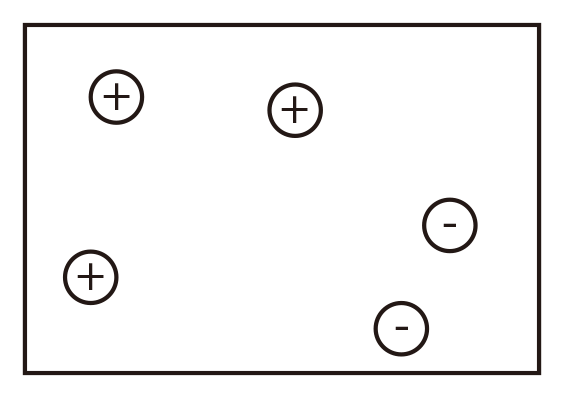
\includegraphics[width= \textwidth]{note2_2_1}
% 		\caption{$n$ small}
% 		\label{fig:side:a}
% 	\end{minipage}%
% 	\begin{minipage}[t]{0.33\linewidth}
% 		\centering
% 		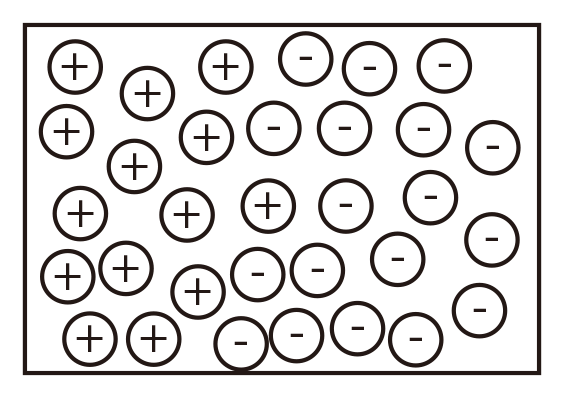
\includegraphics[width= \textwidth]{note2_2_2}
% 		\caption{$n$ large}
% 		\label{fig:side:b}
% 	\end{minipage}
% 	\begin{minipage}[t]{0.33\linewidth}
% 	\centering
% 	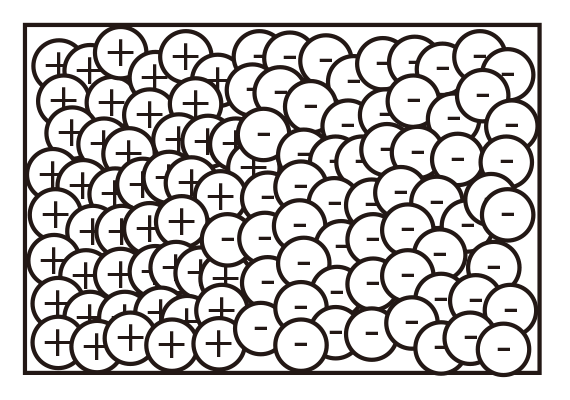
\includegraphics[width= \textwidth]{note2_2_3}
% 	\caption{$n \to \infty$}
% 	\label{fig:side:b}
% \end{minipage}
% \end{figure}
\end{frame}
%------------------------------------------------
\begin{frame}
\frametitle{The Bayesian Way}
A natural choice for the prior P($\theta$) is the Beta distribution:
\begin{align}
P(\theta) = \frac{\theta^{\alpha - 1}(1 - \theta)^{\beta - 1}}{B(\alpha, \beta)}\nonumber
\end{align}
where $B(\alpha, \beta) = \frac{\Gamma(\alpha) \Gamma(\beta)}{\Gamma(\alpha+\beta)}$ is the normalization constant (if this looks scary don't worry about it, it is just there to make sure everything sums to 1 and to scare children at Halloween). Note that here we only need a distribution over a singly binary random variable $\theta$. (The multivariate generalization of the Beta distribution is the Dirichlet distribution.)

\end{frame}
%------------------------------------------------
\begin{frame}
\frametitle{The Bayesian Way}
Why is the Beta distribution a good fit?
\begin{itemize}
	\item it models probabilities $(\theta lives on \left[0,1\right])$
	\item it is of the same distributional family as the binomial distribution (conjugate prior) �� the math will turn out nicely:
\end{itemize}
\begin{align}
P(\theta \mid D) \propto P(D \mid \theta) P(\theta) \propto \theta^{n_H + \alpha -1} (1 - \theta)^{n_T + \beta -1}\nonumber
\end{align}
So far, we have a distribution over $\theta$. How can we get an estimate for $\theta$?
\begin{figure}[h]
	\centering
	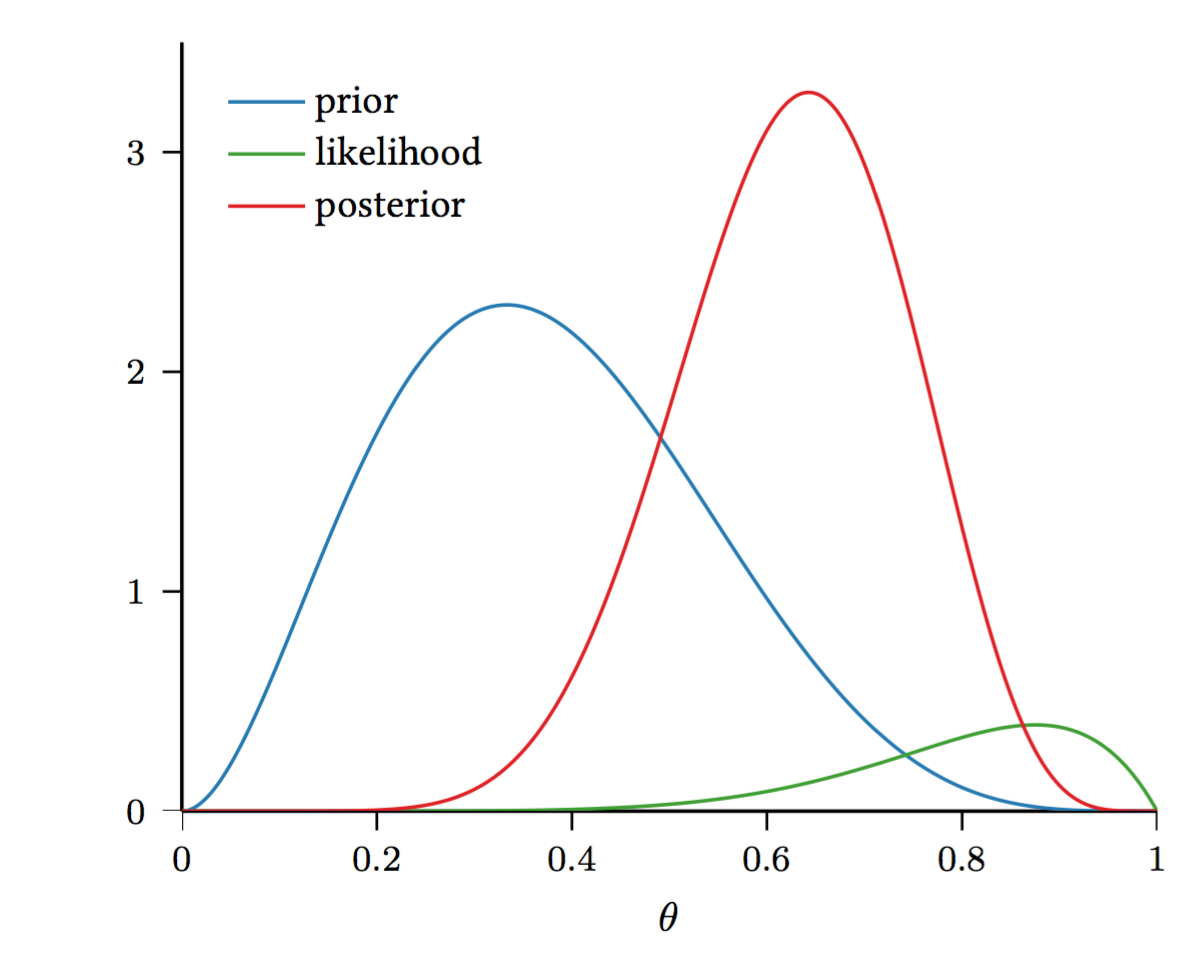
\includegraphics[width=6cm,height=4cm]{BayesianCoinFlipping}
\end{figure}
\end{frame}
%------------------------------------------------
\subsection{Maximum a Posteriori Probability Estimation (MAP)}
\begin{frame}
\frametitle{Maximum a Posteriori Probability Estimation (MAP)}
For example,we can choose $\hat{\theta}$ to be the most likely $\theta$ given the data.
\begin{block}{MAP Principle:Find $\hat{\theta}$ that maximizes the posterior distribution $P(\theta \mid D)$:}
\begin{align}
\hat{\theta}_{MAP} &= \operatorname*{argmax}_{\theta} \,P(\theta \mid D)\nonumber \\
					&= \operatorname*{argmax}_{\theta} \, \log P(D \mid \theta) + \log P(\theta)\nonumber
\end{align}
\end{block}
\end{frame}
%------------------------------------------------
\begin{frame}
\frametitle{Maximum a Posteriori Probability Estimation (MAP)}
For out coin flipping scenario, we get:
\begin{align}
\hat{\theta}_{MAP} &= \operatorname*{argmax}_{\theta} \;P(\theta | Data)\nonumber \\
&= \operatorname*{argmax}_{\theta} \; \frac{P(Data | \theta)P(\theta)}{P(Data)}\qquad\qquad\qquad\qquad  \text{(By Bayes rule)}\nonumber \\
&= \operatorname*{argmax}_{\theta} \;\log(P(Data | \theta)) + \log(P(\theta))\nonumber \\
&= \operatorname*{argmax}_{\theta} \;n_H \cdot \log(\theta) + n_T \cdot \log(1 - \theta) + (\alpha - 1)\cdot \log(\theta) + (\beta - 1) \cdot \log(1 - \theta)\nonumber \\
&= \operatorname*{argmax}_{\theta} \;(n_H + \alpha - 1) \cdot \log(\theta) + (n_T + \beta - 1) \cdot \log(1 - \theta)\nonumber \\
&\Longrightarrow  \hat{\theta}_{MAP} = \frac{n_H + \alpha - 1}{n_H + n_T + \beta + \alpha - 2}\nonumber
\end{align}
\end{frame}
%------------------------------------------------
\begin{frame}
\frametitle{Maximum a Posteriori Probability Estimation (MAP)}
\begin{block}{comments:}
\begin{itemize}
	\item The MAP estimate is identical to MLE with $\alpha-1$ hallucinated heads and $\beta-1$ hallucinated tails
	\item As $n \rightarrow \infty, \hat\theta_{MAP} \rightarrow \hat\theta_{MLE}$ as $\alpha-1$ and $\beta-1$ become irrelevant compared to very large $n_H,n_T$.
	\item MAP is a great estimator if an accurate prior belief is available (and mathematically tractable).
	\item If n is small, MAP can be very wrong if prior belief is wrong!
\end{itemize}
\end{block}
\end{frame}
%%------------------------------------------------
\section{"True" Bayesian approach}
%------------------------------------------------
\subsection{Bayesian approach to make prediction}
\begin{frame}
\frametitle{Bayesian approach to make prediction}
Note that MAP is only one way to get an estimator. There is much more information in $P(\theta \mid D)$, and it seems like a shame to simply compute the mode and throw away all other information. A true Bayesian approach is to use the posterior predictive distribution directly to make prediction about the label Y of a test sample with features X:

$$P(Y\mid D,X) = \int_{\theta}P(Y,\theta \mid D,X) d\theta = \int_{\theta} P(Y \mid \theta, D,X) P(\theta | D) d\theta$$

Unfortunately, the above is generally intractable in closed form and sampling techniques, such as Monte Carlo approximations, are used to approximate the distribution. A pleasant exception are Gaussian Processes, which we will cover later in this course.
\end{frame}
%------------------------------------------------
\begin{frame}
\frametitle{Bayesian approach to make predictions}
Another exception is actually our coin toss example. To make predictions using $\theta$ in our coin tossing example, we can use
\begin{align}
P(heads \mid D) =& \int_{\theta} P(heads, \theta \mid D) d\theta\nonumber\\
 =& \int_{\theta} P(heads \mid \theta, D) P(\theta \mid D) d\theta \nonumber\\ 
 =& \int_{\theta} \theta P(\theta \mid D) d\theta\nonumber\\ 
 =&E\left[\theta|D\right]\nonumber\\
 =&\frac{n_H + \alpha}{n_H + \alpha + n_T + \beta}\nonumber
\end{align}
$$\textrm{(Chain rule: $P(A,B|C)=P(A|B,C)P(B|C)$.)} $$

Here, we used the fact that we defined $P(heads \mid D, \theta)= P(heads \mid \theta)=\theta$ (this is only the case because we assumed that our data is drawn from a binomial distribution - in general this would not hold).
\end{frame}
%%------------------------------------------------
\section{Machine Learning and estimation}
%------------------------------------------------
\subsection{Machine Learning and estimation}
\begin{frame}
\frametitle{Machine Learning and estimation}
In supervised Machine learning you are provided with training data D. You use this data to train a model, represented by its parameters $\theta$. With this model you want to make predictions on a test point $x_t$.
\begin{itemize}	
	\item MLE Prediction: $P(y|x_t;\theta)$ Learning:$\theta=\operatorname*{argmax}_\theta P(D;\theta)$. Here $\theta$ is purely a model parameter.
	\item MAP Prediction: $P(y|x_t,\theta)$ Learning: $\theta=\operatorname*{argmax}_\theta P(\theta|D)\propto P(D \mid \theta) P(\theta)$. Here $\theta$ is a random variable.
	\item "True Bayesian" Prediction: $P(y|x_t,D)=\int_{\theta}P(y|\theta)P(\theta|D)d\theta$. Here $\theta$ is integrated out - our prediction takes all possible models into account.
\end{itemize}
As always the differences are subtle. In MLE we maximize $\log\left[P(D;\theta)\right]$ in MAP we maximize $\log\left[P(D|\theta)\right]+\log\left[P(\theta)\right]$. So essentially in MAP we only add the term $\log\left[P(\theta)\right]$ to our optimization. This term is independent of the data and penalizes if the parameters, $\theta$ deviate too much from what we believe is reasonable. We will later revisit this as a form of regularization, where $\log\left[P(\theta)\right]$ will be interpreted as a measure of classifier complexity.
\end{frame}
%------------------------------------------------
%------------------------------------------------

%%------------------------------------------------

%------------------------------------------------
%%------------------------------------------------
%\section{Reference}
%------------------------------------------------
%\begin{frame}
%\frametitle{Reference}
%\begin{thebibliography}{4}
%\bibitem{LS-SPH} F. Zou, C. Liu, H. Ling, H. Feng, L. Yan, and D. Li, "Least square regularized spectral hashing for similarity search," Signal Processing, vol. 93, pp. 2265-2273, 2013. (SCI,EI)
%\bibitem{KMFH} F. Zou, Y. Chen, J. Song, K. Zhou, Y. Yang, and N. Sebe, "Compact image fingerprint via multiple kernel hashing," IEEE Transactions on Multimedia, vol. 17, pp. 1006-1018, 2015. (SCI,EI)
%\bibitem{KNPH} C. Liu, H. Ling, F. Zou, L. Yan, Y. Wang, H. Feng, et al., "Kernelized neighborhood preserving hashing for social-network-oriented digital fingerprints," IEEE Transactions on Information Forensics and Security, vol. 9, pp. 2232-2247, 2014. (SCI,EI)
%\bibitem{DTSH} Liu, Yu; Song, Jingkuan; Zhou, Ke; Yan, Lingyu; Liu, Li; Zou, Fuhao; Shao, Ling, "Deep Self-taught Hashing for Image Retrieval," IEEE Transactions on Cybernetics, May 3, 2018. (SCI,EI)
%\bibitem{DeepFace} Fuhao Zou, Fan Yang, Wei Chen,Kai Lia, Jingkuan Song, Jingcai Chen, Hefei Ling, "Fast Large Scale Deep Face Search," Pattern Recognition Letters, Januray 3, 2019. (SCI,EI)
%\end{thebibliography}
%\end{frame}
%------------------------------------------------
\begin{frame}
\Huge{\centerline{The End}}
\end{frame}
\end{CJK*}
\end{document}
%\end{document}
